\documentclass[conference]{IEEEtran}
\IEEEoverridecommandlockouts

\usepackage[T1]{fontenc}
\usepackage{amsmath,amssymb}
\usepackage{graphicx}
\usepackage{booktabs}
\usepackage{multirow}
\usepackage{array}
\usepackage{float}
\usepackage[hidelinks]{hyperref}
\usepackage{url}
\usepackage{cite}

\newcommand{\zcoll}{z_{\mathrm{coll}}}
\newcommand{\sighat}{\hat{\sigma}}
\newcommand{\sg}{\operatorname{sg}}
\newcommand{\code}[1]{\texttt{\small #1}}

\begin{document}

\title{SimLingo-Risk: Building and Testing a Collision-Risk Monitor for a Vision--Language--Action Driving Model}

\author{\IEEEauthorblockN{Layan Anabosi, Nawar Sgier, Elad Amrani}
\IEEEauthorblockA{Technion -- Israel Institute of Technology\\
\{sgier.nawar, layananabosi\}@campus.technion.ac.il}}

\maketitle

\begin{abstract}
We built a read-only monitor that displays a collision-hazard score and an
uncertainty estimate next to the outputs of SimLingo, a vision--language--action
(VLA) driving model, in the CARLA simulator. The monitor is a probe with
264K parameters that reads the last hidden state of the frozen model. No SimLingo
weight is changed, and the monitor never affects control. We evaluated it first on
recorded frames and then during simulated drives. On held-out frames, the hazard
score reached an AUROC of 0.960 (mean of five seeds) with an expected calibration
error of 0.014. When a whole scenario type was held out, the AUROC fell to 0.748.
Across 216 Bench2Drive routes driven with the monitor attached, the mean score over
each route reached an AUROC of 0.659 for distinguishing routes that ended in a
collision. Within the 16 collision routes we analyzed around the moment of impact,
the mean frame-level AUROC was 0.504, which is chance level. The monitor told us
more about which routes contained a collision than about when the collision
occurred. Feeding the predicted risk back into action prediction did not reduce
action error.
\end{abstract}

% =====================================================================
\section{Goal and Contribution}
\label{sec:intro}

SimLingo~\cite{renz2025simlingo} drives from front-camera images. For every frame
it produces a planned path, a speed profile, and a sentence of driving commentary.
It won the CARLA Challenge 2024 and reports strong results on
Bench2Drive~\cite{jia2024bench2drive}. Its outputs, however, contain no explicit
statement of how dangerous the scene is (gap G1) and no estimate of how much its
actions can be trusted (gap G2). Danger shows up only indirectly, for example as a
lower target speed or a remark about a pedestrian.

The goal of this project was to find out whether this information can be read from
SimLingo's internal representation, and whether a score built on it is useful while
the car is driving. We trained a small probe on the frozen model's last hidden state
to predict five risk quantities computed from simulator state, together with an
uncertainty for an action estimate. We then ran the same probe live in CARLA as a
monitor that observes the drive without changing it. Two further gaps are outside
our scope: SimLingo's language and actions can disagree (G3), and whatever risk
information the model holds is not stored in a named, separable form (G4).

\emph{Related work.} RiskMonitor~\cite{xiong2025riskmonitor} estimates collision
risk with a plug-in module that reads the planning and motion tokens of end-to-end
planners. SafeAlign-VLA~\cite{tian2026safealign} adds negative, unsafe examples
when aligning a driving VLA. We leave the VLA unchanged and read the hidden state of
its language model. For uncertainty we use the heteroscedastic regression of Kendall
and Gal~\cite{kendall2017uncertainties,kendall2018multitask}, and we compare with
MC-Dropout~\cite{gal2016dropout} and deep
ensembles~\cite{lakshminarayanan2017ensembles}.

\emph{What we built and tested.}
\begin{enumerate}
\item A feature and label pipeline: the last-token hidden state of frozen SimLingo
for 117{,}029 logged frames, and five risk labels computed from the logged simulator
state.
\item A probe with 264{,}489 parameters (0.03\% of the 0.8B-parameter backbone)
that predicts the risk vector and an action uncertainty, trained with five seeds.
\item A live monitor inside the CARLA closed loop. SimLingo's driving code path does
not produce the hidden state we trained on, so the monitor runs its own forward pass
at every simulator tick (Sec.~\ref{sec:monitor}).
\item An evaluation on held-out frames, on held-out scenario types, and on 216
Bench2Drive routes at route and frame level. Two of the results are negative, and we
report them.
\end{enumerate}

% =====================================================================
\section{System Design}
\label{sec:design}

\subsection{SimLingo}

SimLingo~\cite{renz2025simlingo} is built on InternVL2-1B. An InternViT-300M encoder
turns two $448{\times}448$ front-camera tiles into 512 visual tokens. These are
interleaved with a navigation goal and a language prompt and passed to a
Qwen2-0.5B language model, which the original authors fine-tuned with LoRA. Learned
query tokens appended to the sequence are decoded by two small MLPs into geometric
path waypoints $\mathbf{p}$ (one point per metre), which set the steering target,
and temporal speed waypoints $\mathbf{w}$ (one point every 0.25\,s), which set the
target speed. Two PID controllers convert these into steering and acceleration; the
model never outputs steering or throttle directly. A language head produces the
commentary. We use the released weights (0.8B parameters) without modification.
Fig.~\ref{fig:arch} shows where our probe attaches.

\begin{figure}[t]
\centering
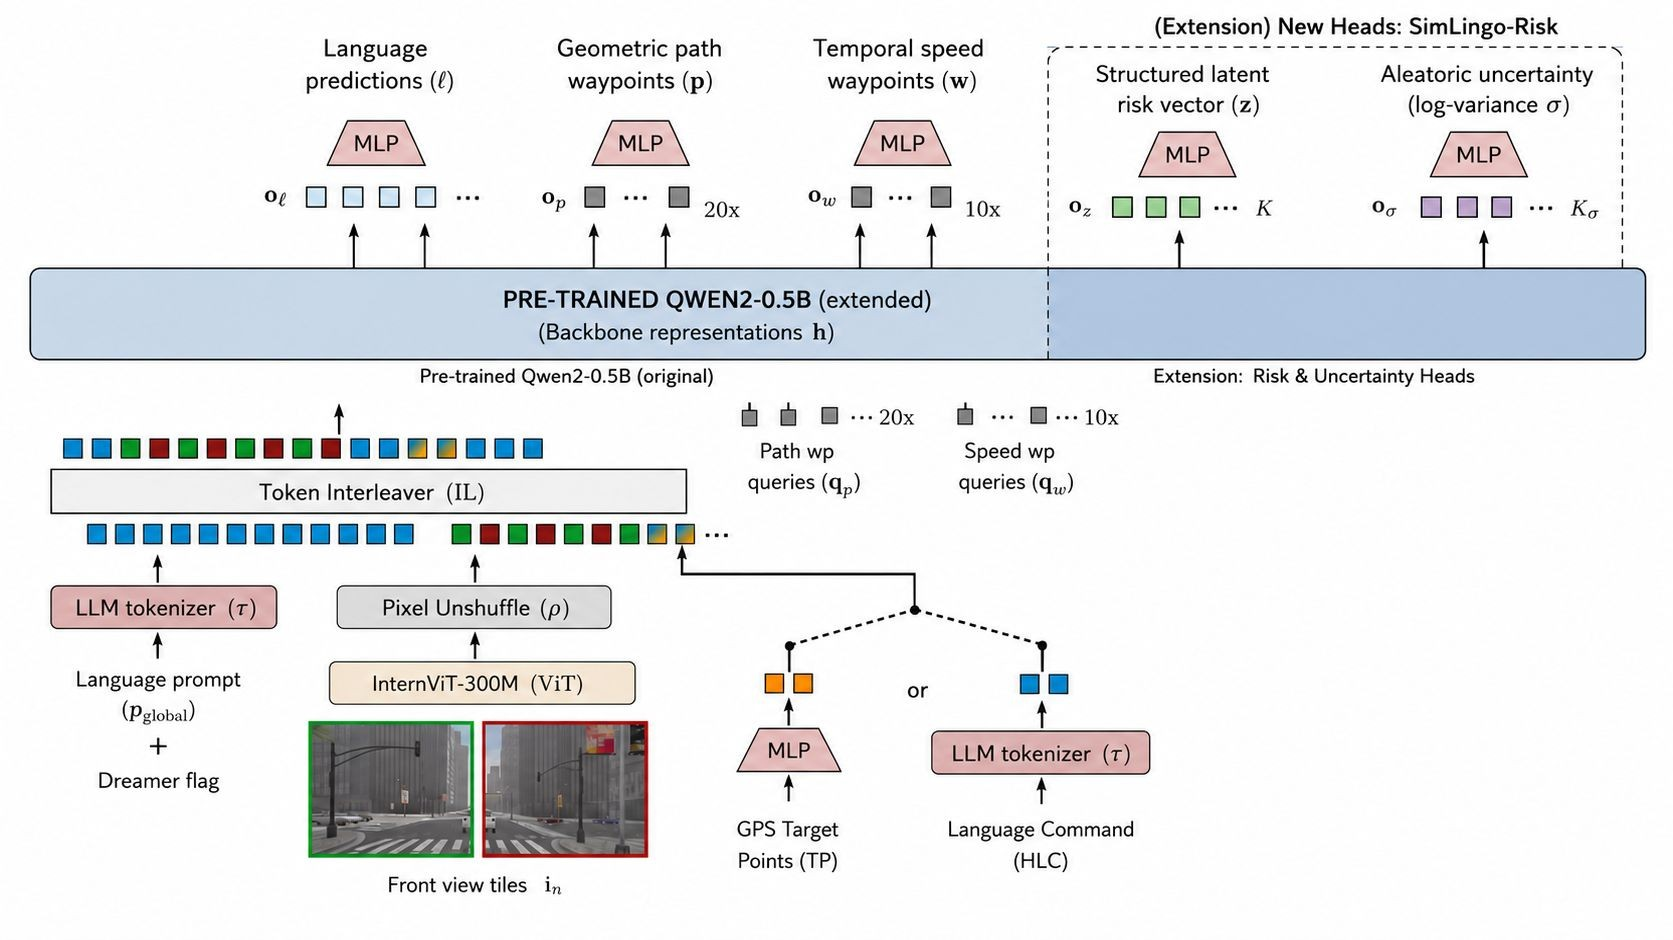
\includegraphics[width=\columnwidth]{figures/architecture.jpg}
\caption{SimLingo with the SimLingo-Risk extension. Left: the original frozen model,
whose Qwen2 backbone produces language, path waypoints $\mathbf{p}$ and speed
waypoints $\mathbf{w}$. Right (dashed): our probe reads the backbone
representation $\mathbf{h}$ and outputs the risk vector $\mathbf{z}$ and an
action log-variance. Adapted from~\cite[Fig.~1]{renz2025simlingo}.}
\label{fig:arch}
\end{figure}

\begin{figure*}[t]
\centering
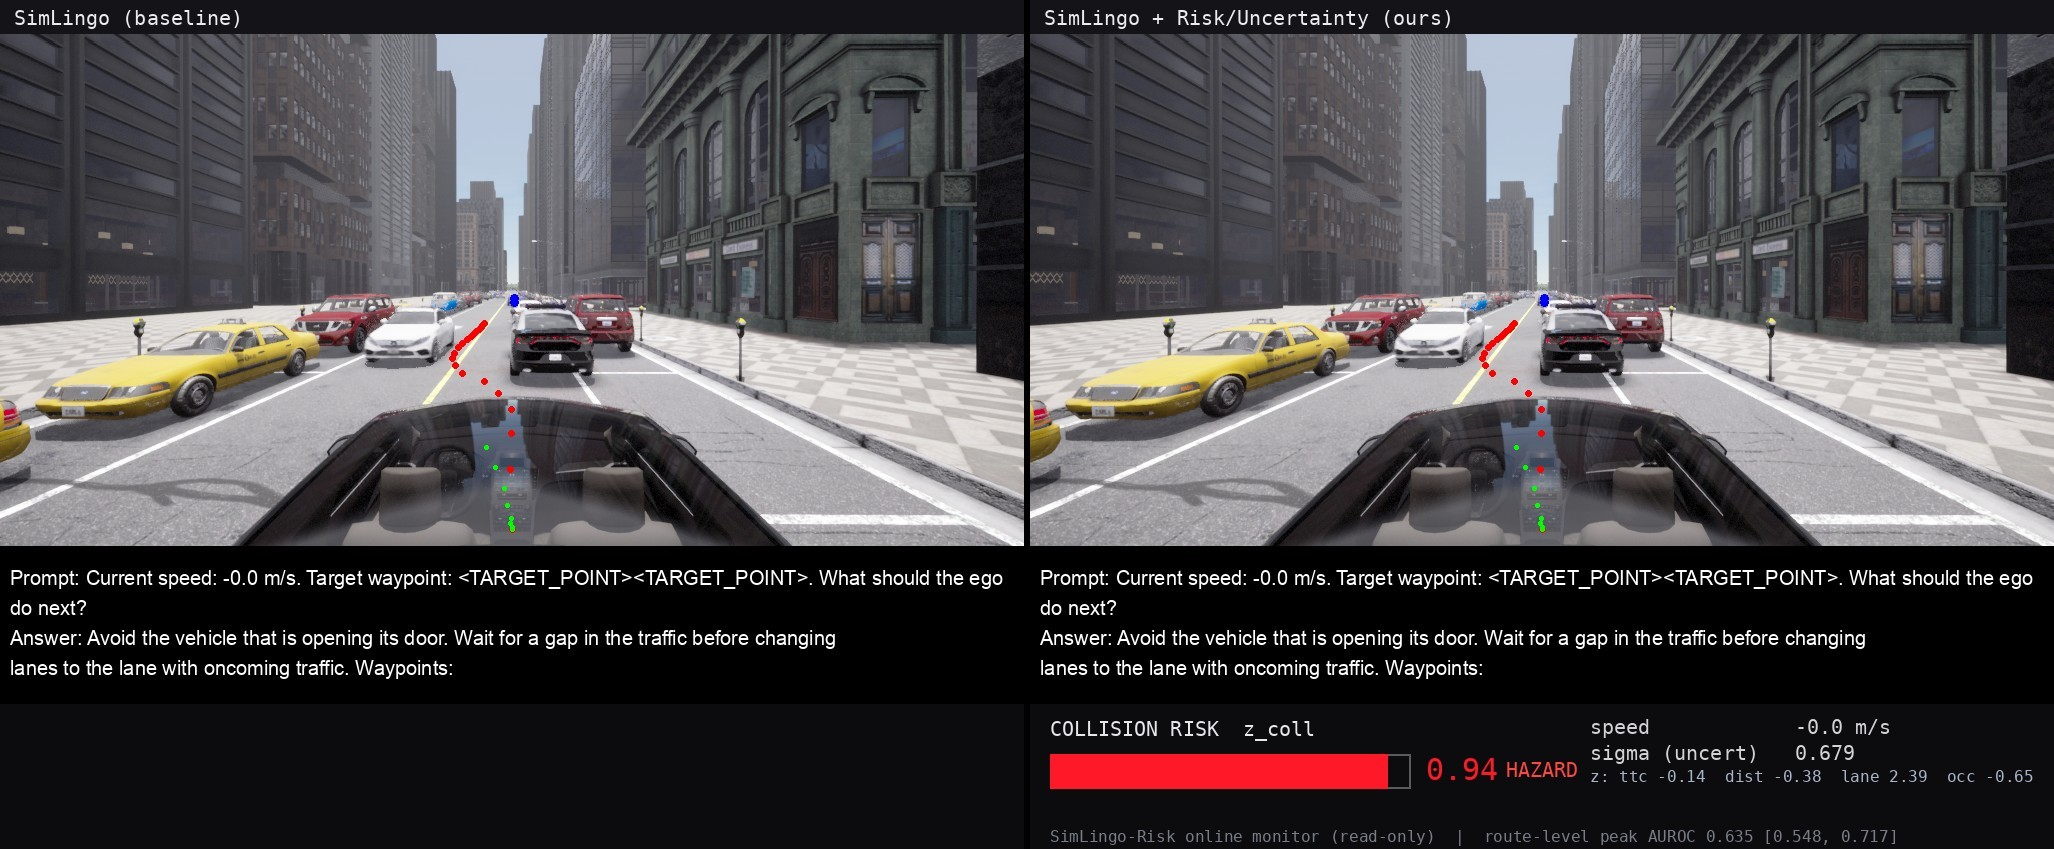
\includegraphics[width=\textwidth]{figures/door.jpg}
\caption{Reading the monitor. Left: SimLingo as published. Right: the same
closed-loop run with the monitor attached. The camera view, planned path, prompt and
SimLingo's answer are identical in both panes because the monitor does not affect
control. The overlay at the bottom right shows $\zcoll$ (bar), ego speed, $\sighat$
and the four continuous coordinates of $\hat{\mathbf{z}}$ in standardized units. In
this frame a parked car opens its door ahead and SimLingo has to change into the
oncoming lane. The monitor reports $\zcoll=0.94$ and $\sighat=0.679$, the highest
uncertainty among our examples.}
\label{fig:door}
\end{figure*}

\subsection{The hidden-state feature}

For each frame we take the adaptor feature at the last token position,
\code{adaptor\_features[0,-1,:]}, a vector $\mathbf{h}\in\mathbb{R}^{896}$. In a
causal model this position has attended to every visual, prompt and goal token, and
it is the summary that the action heads consume. We use the last token instead of
mean or max pooling so that the feature seen in training is exactly the one
available at run time. A cache of full sequences and a cache of last tokens gave
bit-identical features. The probe receives $\mathbf{h}$ without normalization;
only the regression targets are standardized. As a check on the pipeline, an
independent reimplementation of the probe reached a held-out AUROC of 0.966,
against 0.960 for the main pipeline.

$\mathbf{h}$ is a deterministic function of the image, prompt, goal and checkpoint.
It is computed from pixels and contains no simulator state directly, and no single
dimension has an assigned meaning.

\subsection{Risk targets}

The probe predicts $\mathbf{z}\in\mathbb{R}^5$ (Table~\ref{tab:z}). We computed
each coordinate with a label function of our own from the state stored with every
frame of SimLingo's driving logs: object boxes, ego state, route and hazard flags.
No new simulator rollouts or human annotation were needed. We call the results
pseudo-labels, because they are simulator quantities passed through definitions we
chose; a different definition of occlusion, for example, would give a different
target. A high AUROC therefore shows that $\mathbf{h}$ contains what our label
functions measure, not risk in a general sense. In return the labels are dense,
deterministic and synchronized exactly with $\mathbf{h}$, since both come from the
same simulator tick.

\begin{table}[t]
\centering
\caption{Risk outputs, in the order of the trained head. C = continuous
(MSE loss), B = binary (BCE loss). The monitor's hazard score is
$\zcoll=\mathrm{sigmoid}(\hat z_5)$.}
\label{tab:z}
\footnotesize
\setlength{\tabcolsep}{3pt}
\begin{tabular}{@{}l p{5.3cm} c@{}}
\toprule
Output & Label rule & Type \\
\midrule
$z_1$ inverse TTC & Closing speed divided by range to the nearest vehicle or
pedestrian, clipped to $[0,3]\,\mathrm{s}^{-1}$; 0 if it is moving away & C \\
$z_2$ distance & Planar range to the nearest vehicle or pedestrian; 75\,m if none &
C \\
$z_3$ lane offset & Perpendicular distance from the ego vehicle to the line through
the first two route points & C \\
$z_4$ occlusion & Fraction of nearby agents with no recorded sensor points & C \\
$z_5$ collision hazard & 1 if the logged \code{vehicle\_hazard} or
\code{walker\_hazard} flag is set & B \\
\bottomrule
\end{tabular}
\end{table}

Two definitions matter for reading the results. First, $z_5$ is a hazard flag,
not an impact. A frame is positive when the logged measurements mark a vehicle or a
pedestrian as a hazard. Physical contact is a separate and much rarer event, which
we use only in the closed-loop evaluation (Sec.~\ref{sec:res-online}). Second, we
regress inverse time-to-collision because TTC is unbounded when nothing is closing,
and an unbounded target destabilizes the loss.

\subsection{Probe and training objective}

The probe has a shared trunk,
$\mathrm{Linear}(896{\to}256)\to\mathrm{GELU}\to\mathrm{LayerNorm}\to
\mathrm{Linear}(256{\to}128)\to\mathrm{GELU}$, with output $\mathbf{t}\in
\mathbb{R}^{128}$, followed by three linear heads. The risk head maps $\mathbf{t}$
to $\hat{\mathbf{z}}\in\mathbb{R}^5$. An action-mean head and a log-variance head
each map $[\mathbf{t};\sg(\hat{\mathbf{z}})]\in\mathbb{R}^{133}$ to three outputs,
where $\sg$ is a stop-gradient: the uncertainty head can use the risk estimate but
does not train it. In total the probe has 264{,}489 parameters.

\emph{Risk loss.} With $\tilde{\mathbf{z}}$ the pseudo-labels,
\begin{equation}
L_z=\sum_{k\in\{1,2,3,4\}}(\hat z_k-\tilde z_k)^2+\mathrm{BCE}(\hat z_5,\tilde z_5).
\end{equation}

\emph{Uncertainty loss.} For each frame the action target is
$\mathbf{y}=(x_{\mathrm{aim}},y_{\mathrm{aim}},v_{\mathrm{target}})$: the aim point
that SimLingo's lateral controller steers toward, taken from the path waypoints, and
the target speed, taken from the speed waypoints, as recorded for that frame. The
mean head predicts $\hat{\boldsymbol\mu}$ and the log-variance head predicts
$\hat s_c=\log\sighat_c^2$ for each component $c$. Following Kendall and
Gal~\cite{kendall2017uncertainties}, we minimize the heteroscedastic Gaussian
negative log-likelihood
\begin{equation}
L_\sigma=\tfrac12\sum_{c=1}^{3}\Big[e^{-\hat s_c}(\hat\mu_c-y_c)^2+\hat s_c\Big].
\end{equation}
The first term lets the model accept large errors on frames it marks as uncertain;
the second keeps it from marking every frame as uncertain. For a fixed
$\hat\mu_c$ the loss is smallest when $\sighat_c^2$ equals the squared residual
$(\hat\mu_c-y_c)^2$, so no uncertainty label is needed. We report
$\sighat=\frac13\sum_c\exp(\hat s_c/2)$. The full objective is
$L=L_z+\lambda_\sigma L_\sigma$. Only probe parameters are trained.

\emph{What $\sighat$ measures.} $\sighat$ predicts the error of the probe's own
mean head $\hat{\boldsymbol\mu}$, which reads the same hidden state as SimLingo's
action heads. It is therefore not a direct estimate of SimLingo's closed-loop driving
error. We use it as an indicator of how hard a frame is to act on from
$\mathbf{h}$. The correlation in Sec.~\ref{sec:res-offline} is computed between
$\sighat$ and the realized residual $r=\lVert\mathbf{y}-\hat{\boldsymbol\mu}\rVert$
on held-out frames. $\sighat$ is an aleatoric estimate: it models ambiguity in the
frame, such as occlusion or several acceptable actions. Epistemic estimates require
many passes or models per frame, so we use them only as baselines.

Risk and uncertainty are separate outputs because they can disagree. A construction
site can be clearly dangerous while the required action is obvious, and following a
car at speed can be low-risk while the action is less certain
(Fig.~\ref{fig:axes} in the Appendix).

\emph{Training.} Features are extracted once and cached. Each run trains for 10
epochs on the training split only, with no early stopping, no model selection on the
validation split and no hyperparameter sweep. A run takes about two hours on one
A100 GPU. Every result is repeated over five seeds.

\subsection{Live monitor}
\label{sec:monitor}

The monitor wraps the driving agent without modifying it. One engineering problem
shaped its design. SimLingo drives with \code{predict\_language=True}, which runs
the autoregressive language branch and never calls \code{forward\_model}, the
function that produced our cached features. During driving, the feature
$\mathbf{h}$ we trained on is therefore never computed. The monitor runs its own
forward pass on the same inputs at every simulator tick, extracts the last-token
feature exactly as in the offline pipeline, applies the frozen probe, and logs
$\zcoll$, $\sighat$ and the raw $\hat{\mathbf{z}}$. It draws these values as an
overlay (Fig.~\ref{fig:door}) and never writes to the controller.

CARLA runs in synchronous mode at 20 ticks per simulated second, and the monitor
produces one update per tick. We did not measure the wall-clock cost of the extra
forward pass, so we make no real-time claim.

% =====================================================================
\section{Data and Evaluation}
\label{sec:eval}

\subsection{Data}

All offline training uses SimLingo's existing driving logs. After features and labels
are joined on route and frame, the cache holds 117{,}029 frames from 1{,}282 routes
in seven scenario groups (Appendix, Table~\ref{tab:data}). The groups are uneven:
noScenarios contributes 28{,}965 frames and VehicleTurning only 2{,}470 (2.1\%).
We split the cache into training, validation and test sets with a test fraction of
0.2. All offline numbers are reported on the test split; the validation split serves
only as a cross-check. Consecutive frames of one drive are strongly correlated, so a
held-out split of frames is an in-distribution test. Leave-one-scenario-out
evaluation, which holds out every frame of one scenario group, is the stricter test.
Labels are used only as targets, never as inputs.

Hazard-positive frames are a minority (11.5\% of training frames and 2.0\% of
validation frames in the pilot split of Appendix~\ref{app:pilot}), so we measure
ranking with AUROC instead of accuracy.

\subsection{Experiments}

Table~\ref{tab:exp} lists the completed experiments. A0 is SimLingo with nothing
attached. A2 trains the risk head alone, A3 the uncertainty head alone, and A4 both
jointly; A4 is the main model. A5 compares the action-mean head with and without
$\hat{\mathbf{z}}$ as an input. A7 and A8 are generic uncertainty baselines on the
same frozen $\mathbf{h}$. Two planned experiments were not run: A1, which would
replace the structured $\mathbf{z}$ with an unstructured or random vector of the same
width, and A6, LoRA fine-tuning of the backbone, which did not fit our compute
budget.

\begin{table}[t]
\centering
\caption{Completed experiments. Offline results are on the held-out test split,
mean over five seeds where available.}
\label{tab:exp}
\footnotesize
\setlength{\tabcolsep}{3pt}
\begin{tabular}{@{}l l l@{}}
\toprule
ID & Configuration & Main result \\
\midrule
A0 & SimLingo, nothing attached & DS 88.99 \\
A2 & Risk head only & Hazard AUROC $\approx$0.96 \\
A3 & Uncertainty head only & $\mathrm{corr}(\sighat,r)\approx0.80$ \\
A4 & Joint risk + uncertainty (main) & AUROC 0.9596, ECE 0.0142 \\
A5 & A4, action head with/without $\hat{\mathbf{z}}$ & No change in MSE \\
A7 & MC-Dropout, 20 passes & AUROC 0.616 \\
A8 & Deep ensemble, $K=8$ & AUROC 0.700 \\
LOSO & A4, one scenario group held out & AUROC 0.748 \\
Online & A4 live in CARLA, 216 routes & Route AUROC 0.659 \\
\bottomrule
\end{tabular}
\end{table}

\subsection{Metrics}

Offline, we report AUROC and expected calibration error (ECE)~\cite{guo2017calibration}
for the hazard output, $R^2$ for the continuous coordinates, the correlation between
$\sighat$ and the realized residual $r$, and the coverage of $\sighat$ intervals.
AUROC is unchanged by any monotone rescaling, so a model can rank frames well and
still give poorly calibrated probabilities; we therefore report AUROC and ECE
together. In closed loop, we report route-level AUROC of the peak and of the mean
$\zcoll$ along each route, with 95\% bootstrap intervals (5{,}000 resamples over
routes), and frame-level AUROC around the impact. Driving quality is measured with
the Bench2Drive driving score (DS), route completion (RC) and infraction score (IS);
DS is the per-route product of RC and IS, averaged over routes.

\subsection{Closed-loop protocol}

We used CARLA 0.9.15~\cite{dosovitskiy2017carla} in synchronous mode at 20 ticks per
second, on the 220 short routes of Bench2Drive~\cite{jia2024bench2drive}. Each route
has a start, a goal and one scripted scenario. A full pass takes 14--18\,h per
configuration. We ran A0 and A0 with the monitor attached. Some routes reached the
wall-clock limit and were re-run. The online analysis uses the 216 routes with
complete monitor logs; according to the evaluator, 46 of them contained a collision.
Route outcome is used only as the answer key.

The frame-level analysis covers 16 of the 46 collision routes. On each, we located
the collision frame $j$ from the evaluator's collision position, which matched a
logged ego position to 0.00\,m, and labeled frames $j-3$ to $j+12$ as positive. At
20\,Hz this window runs from 0.15\,s before contact to 0.6\,s after it, so it tests
whether the score reacts around the impact. It does not test early warning.

% =====================================================================
\section{Results}
\label{sec:results}

\subsection{Offline hazard ranking and calibration}
\label{sec:res-offline}

On the held-out test split, the A4 hazard head reached AUROC $0.9596\pm0.0010$ with
ECE $0.0142\pm0.0078$ (mean $\pm$ population standard deviation over five seeds,
Table~\ref{tab:offline}). Per-seed AUROC ranged from 0.9583 to 0.9608. ECE varied
more between seeds, so we report its spread instead of a single value. The
validation split gave nearly the same values. The deployed monitor uses seed~0,
whose AUROC (0.9595) is closest to the mean; it is not the best seed. The
uncertainty $\sighat$ correlated with the realized residual at $0.80$.

\begin{table}[t]
\centering
\caption{A4 probe offline. Mean $\pm$ std over five seeds.}
\label{tab:offline}
\footnotesize
\begin{tabular}{@{}l c c@{}}
\toprule
Metric & Test (reported) & Validation (check) \\
\midrule
Hazard AUROC $\uparrow$ & $0.9596\pm0.0010$ & $0.9599\pm0.0021$ \\
Hazard ECE $\downarrow$ & $0.0142\pm0.0078$ & $0.0098\pm0.0025$ \\
$\mathrm{corr}(\sighat, r)$ $\uparrow$ & $0.7966\pm0.0118$ & $0.7794\pm0.0314$ \\
\bottomrule
\end{tabular}
\end{table}

Generic uncertainty computed from the same features ranks hazard frames much less
well (Table~\ref{tab:baselines}). No epistemic, aleatoric or total score from
MC-Dropout or the ensemble exceeds 0.73. These estimates indicate that a frame is
hard to predict; they are not trained to indicate a hazard. The baselines were scored
on different frame sets from the probe, so the gap is large but not a matched
comparison.

\begin{table}[t]
\centering
\caption{Hazard AUROC of generic uncertainty on the same frozen $\mathbf{h}$ and of
the supervised hazard head. The rows use different frame sets, so the comparison is
qualitative.}
\label{tab:baselines}
\footnotesize
\setlength{\tabcolsep}{3pt}
\begin{tabular}{@{}l c c r c c c@{}}
\toprule
Method & Labels & Passes & Frames & Epist. & Aleat. & Total \\
\midrule
Chance & -- & -- & -- & -- & -- & 0.500 \\
MC-Dropout (A7) & no & 20 & 4{,}500 & 0.573 & 0.589 & 0.616 \\
Ensemble (A8) & no & 8 & 23{,}057 & 0.722 & 0.697 & 0.700 \\
Probe $\zcoll$ (A4) & yes & 1 & test split & -- & -- & \textbf{0.960} \\
\bottomrule
\end{tabular}
\end{table}

\subsection{Which risk coordinates the probe recovers}

Geometric quantities were recovered better than dynamic ones (Appendix,
Table~\ref{tab:r2}). Lane offset had the highest $R^2$ ($\approx0.87$), followed by
nearest-agent distance ($\approx0.80$). The occlusion proxy reached $\approx0.50$.
Inverse TTC was the hardest ($\approx0.30$). A single frame shows how far away
objects are more clearly than how fast they are approaching, and this label, derived
from the nearest agent's relative motion, is also the noisiest.

\subsection{Calibrating the uncertainty}

The raw path uncertainty was over-confident: 30.1\% of held-out residuals fell within
$\pm1\sighat$, against 68.3\% for a calibrated Gaussian. A single recalibration
factor, $\tau=4.10$, fitted on held-out data, raised one-sigma coverage to 74.5\%,
slightly above nominal (Appendix, Table~\ref{tab:coverage}). Because $\tau$
rescales $\sighat$ monotonically, the ranking of frames and the
$\sighat$--$r$ correlation do not change. At $3\sighat$ the recalibrated coverage is
0.971 against 0.997, which is consistent with path errors that have heavier tails
than a Gaussian.

\subsection{Feeding risk back into action prediction (A5)}

Giving the action-mean head $\hat{\mathbf{z}}$ as an extra input did not reduce
action error. In the single comparison we report, action MSE moved from 0.2609 to
0.2601, a difference of 0.0008. Over five seeds the mean change was
$+0.006\pm0.012$. The two figures come from different runs; both are small
compared with the seed-to-seed spread, and the five-seed interval contains zero. A
likely explanation, which we did not test, is that $\hat{\mathbf{z}}$ is computed
from the same $\mathbf{h}$ the heads already read and adds no new information.

\subsection{Unseen scenario types}

The in-distribution AUROC overstates what the probe achieves on a new type of
hazard. When we trained on six scenario groups and tested on the seventh, hazard
AUROC averaged $0.748\pm0.071$ over the seven folds, about 0.21 lower (Appendix,
Table~\ref{tab:loso}). The folds ranged from 0.848 (SignalizedJunctionRight) to
0.628 (VehicleTurning). Distance transferred best (mean $R^2\approx0.61$). Lane
offset was unstable, with negative $R^2$ on three folds, and inverse TTC did not
transfer ($R^2\approx0$). An early pilot that held out five whole VehicleTurning
routes gave a similar picture: hazard AUROC 0.595 on 549 frames with 11 positives
(Appendix~\ref{app:pilot}).

\subsection{The monitor in closed loop}
\label{sec:res-online}

Table~\ref{tab:online} summarizes the live results.

\begin{table}[t]
\centering
\caption{The frozen probe run live in CARLA. Route-level intervals are 95\%
bootstrap intervals over routes.}
\label{tab:online}
\footnotesize
\setlength{\tabcolsep}{3pt}
\begin{tabular}{@{}l l l@{}}
\toprule
Test & Data & AUROC \\
\midrule
Route, peak $\zcoll$ & 216 routes, 46 with collision & 0.635 [0.548, 0.717] \\
Route, mean $\zcoll$ & 216 routes, 46 with collision & 0.659 [0.570, 0.743] \\
Frame, pooled & frames of 16 collision routes & 0.43 \\
Frame, within route & 16 collision routes & 0.504 (median 0.494) \\
\bottomrule
\end{tabular}
\end{table}

\emph{Route level.} The peak $\zcoll$ on each route separated collision routes from
the others with AUROC 0.635, and the route mean did slightly better, 0.659. Both
intervals exclude 0.5, so a probe trained only on logged frames carries information
about which live routes end in a collision. Three factors can explain the drop from
the offline figure. In closed loop each action changes the next image, so the frames
drift away from the logged data. The target changes from a hazard flag to an actual
collision. With one scripted scenario per route there are only 46 positive routes,
which leaves wide intervals.

\emph{Frame level.} Pooling the frames of the 16 analyzed routes gave AUROC 0.43,
below chance. On busy routes $\zcoll$ stays around 0.6--0.9 throughout, so no single
threshold separates frames across routes. We therefore ranked each route's impact
frames against that route's other frames. The resulting within-route AUROC was 0.504
(median 0.494), which is chance level. The routes split into two groups: the score
rose around the impact on 6 of the 16 routes (AUROC 0.60--0.86) and fell on 6
(0.19--0.40). We did not tune the window. The probe reflects whether a route is
dangerous; it does not mark the moment of impact.

\emph{Qualitative behavior.} On the scenes we inspected, the overlay reports high
hazard for pedestrians in the path by day and at night and for a parked vehicle in
fog (Fig.~\ref{fig:door} and Appendix, Fig.~\ref{fig:live}). In each case SimLingo's
own answer already names the hazard, for example ``Remain stopped due to the
pedestrian''; the monitor turns that into a number with an uncertainty attached.
These are selected examples and do not replace the statistics above.

\emph{Driving score.} Table~\ref{tab:ds} lists the driving scores. A0 scored DS
88.99 and the monitored run 88.02. Each configuration was run once, and the
across-route standard deviation of DS is 18.46, so these two runs cannot attribute
the difference of 0.97 to a cause. In side-by-side recordings the trajectories and
SimLingo's commentary are identical with and without the monitor
(Fig.~\ref{fig:door}). Our A0 figure comes from one evaluation of the released
checkpoint, while the published figure is a mean over three training seeds, so the
two are not directly comparable.

\begin{table}[t]
\centering
\caption{Closed-loop driving on Bench2Drive.}
\label{tab:ds}
\footnotesize
\begin{tabular}{@{}l c c c@{}}
\toprule
Configuration & DS & RC & IS \\
\midrule
Published SimLingo~\cite{renz2025simlingo}$^\dagger$ & $85.07\pm0.95$ & -- & -- \\
A0, our run$^\ddagger$ & 88.99 & 99.31 & 0.895 \\
A0 + read-only monitor & 88.02 & -- & -- \\
\bottomrule
\multicolumn{4}{@{}p{0.95\columnwidth}@{}}{\scriptsize $^\dagger$From
\cite[Table~2]{renz2025simlingo}: mean over three training seeds, with the
minimum-speed penalty ignored in DS. $^\ddagger$Across-route standard deviation of
DS: 18.46. --: not reported.}
\end{tabular}
\end{table}

% =====================================================================
\section{Limitations and Conclusion}
\label{sec:limits}

\emph{Limitations.} We do not claim that SimLingo-Risk makes a car safer. The monitor
is read-only by construction, and the one experiment that fed risk back into action
prediction (A5) found no effect. Testing an intervention, such as an emergency-brake
fallback on the riskiest frames measured by collisions avoided against intervention
rate, is future work. The targets are simulator pseudo-labels that we defined, and
the hazard flag we trained on is not the same event as a collision. The offline
AUROC does not carry over to new scenario types (0.960 to 0.748, worst fold 0.628).
Online, the route-level signal is modest, and the frame-level result is at chance;
it was measured on 16 of the 46 collision routes, and its window tests the reaction
around impact, not early warning. Each closed-loop configuration was run once. The
uncertainty baselines were scored on different frame sets, and we did not compute
average precision (AUPRC) for the A4 probe, which would be more informative than
AUROC at low prevalence. We also did not run the controls of A1, LoRA fine-tuning
(A6), monitors built on SimLingo's own outputs (predicted speed, a time-to-collision
from its waypoints, keywords in its commentary), a RiskMonitor-style
probe~\cite{xiong2025riskmonitor}, or a privileged-state upper bound. Finally, the
probe reads a single frame. The frame-level failure suggests that a temporal window
over several consecutive hidden states is the first experiment to try.

\emph{Conclusion.} The last hidden state of a frozen SimLingo contains enough
information for a 264K-parameter probe to rank hazard frames well offline (AUROC
0.960) with nearly calibrated probabilities, and to estimate an uncertainty that
tracks the error of an action estimate read from the same state (correlation 0.80).
Run live in CARLA without touching control, the same probe distinguished routes that
ended in a collision from the others (AUROC 0.659), but it did not locate the moment
of impact within a route (0.504). Feeding the risk back into action prediction did
not help. SimLingo-Risk is useful as a route-level risk indicator. Using it to act,
and making it sensitive to timing, are the next steps.

% =====================================================================
\section*{Project Materials}

Project page with the demonstration video:
\url{https://nawar21.github.io/SimLingoRisk-/}.
Repository with this report and its figures:
\url{https://github.com/nawar21/SimLingoRisk-}.
Code will be released publicly.

% =====================================================================
\begin{thebibliography}{10}

\bibitem{renz2025simlingo}
K.~Renz, L.~Chen, E.~Arani, and O.~Sinavski, ``SimLingo: Vision-only closed-loop
autonomous driving with language-action alignment,'' in \emph{Proc. IEEE/CVF Conf.
Comput. Vis. Pattern Recognit. (CVPR)}, 2025, arXiv:2503.09594.

\bibitem{tian2026safealign}
K.~Tian, Y.~Lian, K.~Yang, X.~Chen, and S.~Li, ``SafeAlign-VLA: A negative-enhanced
safe alignment framework for risk-aware autonomous driving,'' arXiv:2605.19524,
2026.

\bibitem{xiong2025riskmonitor}
Z.~Xiong, S.~Liu, N.~Helgesen, H.~Li, J.~Johnander, and P.-E. Forss\'en,
``Collision risk estimation via loss prediction in end-to-end autonomous driving,''
arXiv:2503.07425, 2025.

\bibitem{kendall2017uncertainties}
A.~Kendall and Y.~Gal, ``What uncertainties do we need in Bayesian deep learning for
computer vision?'' in \emph{Proc. Adv. Neural Inf. Process. Syst. (NeurIPS)}, 2017.

\bibitem{kendall2018multitask}
A.~Kendall, Y.~Gal, and R.~Cipolla, ``Multi-task learning using uncertainty to weigh
losses for scene geometry and semantics,'' in \emph{Proc. IEEE Conf. Comput. Vis.
Pattern Recognit. (CVPR)}, 2018.

\bibitem{gal2016dropout}
Y.~Gal and Z.~Ghahramani, ``Dropout as a Bayesian approximation: Representing model
uncertainty in deep learning,'' in \emph{Proc. Int. Conf. Mach. Learn. (ICML)},
2016.

\bibitem{lakshminarayanan2017ensembles}
B.~Lakshminarayanan, A.~Pritzel, and C.~Blundell, ``Simple and scalable predictive
uncertainty estimation using deep ensembles,'' in \emph{Proc. Adv. Neural Inf.
Process. Syst. (NeurIPS)}, 2017.

\bibitem{guo2017calibration}
C.~Guo, G.~Pleiss, Y.~Sun, and K.~Q. Weinberger, ``On calibration of modern neural
networks,'' in \emph{Proc. Int. Conf. Mach. Learn. (ICML)}, 2017.

\bibitem{dosovitskiy2017carla}
A.~Dosovitskiy, G.~Ros, F.~Codevilla, A.~L\'opez, and V.~Koltun, ``CARLA: An open
urban driving simulator,'' in \emph{Proc. Conf. Robot Learn. (CoRL)}, 2017.

\bibitem{jia2024bench2drive}
X.~Jia, Z.~Yang, Q.~Li, Z.~Zhang, and J.~Yan, ``Bench2Drive: Towards multi-ability
benchmarking of closed-loop end-to-end autonomous driving,'' in \emph{Proc. Adv.
Neural Inf. Process. Syst. (NeurIPS) Datasets and Benchmarks Track}, 2024.

\end{thebibliography}

% =====================================================================
\appendix
\renewcommand{\thetable}{A\arabic{table}}
\renewcommand{\thefigure}{A\arabic{figure}}
\renewcommand{\theHtable}{A\arabic{table}}
\renewcommand{\theHfigure}{A\arabic{figure}}
\setcounter{table}{0}
\setcounter{figure}{0}

\subsection{Data by scenario group}

\begin{table}[H]
\centering
\caption{Frames in the feature cache by scenario group (117{,}029 frames, 1{,}282
routes).}
\label{tab:data}
\footnotesize
\begin{tabular}{@{}l r r@{}}
\toprule
Scenario group & Frames & Share \\
\midrule
noScenarios & 28{,}965 & 24.8\% \\
DynamicObjectCrossing & 23{,}403 & 20.0\% \\
SignalizedJunctionRight & 17{,}834 & 15.2\% \\
ControlLoss & 17{,}041 & 14.6\% \\
SignalizedJunctionLeft & 15{,}694 & 13.4\% \\
OppositeVehicleRunningRedLight & 11{,}622 & 9.9\% \\
VehicleTurning & 2{,}470 & 2.1\% \\
\midrule
Total & 117{,}029 & 100\% \\
\bottomrule
\end{tabular}
\end{table}

\subsection{Per-coordinate recovery}

\begin{table}[H]
\centering
\caption{$R^2$ of $\hat z_k$ against the pseudo-label on the held-out test split
(A4), continuous coordinates.}
\label{tab:r2}
\footnotesize
\begin{tabular}{@{}l c@{}}
\toprule
Coordinate & $R^2$ \\
\midrule
$z_3$ lane offset & $\approx0.87$ \\
$z_2$ nearest-agent distance & $\approx0.80$ \\
$z_4$ occlusion proxy & $\approx0.50$ \\
$z_1$ inverse TTC & $\approx0.30$ \\
\bottomrule
\end{tabular}
\end{table}

\subsection{Coverage of the path uncertainty}

\begin{table}[H]
\centering
\caption{Fraction of held-out residuals inside $\pm k\sighat$, before and after
recalibration with $\tau=4.10$.}
\label{tab:coverage}
\footnotesize
\begin{tabular}{@{}c c c c@{}}
\toprule
Interval & Gaussian & Raw & Recalibrated \\
\midrule
$0.5\sighat$ & 0.383 & 0.155 & 0.508 \\
$1.0\sighat$ & 0.683 & 0.301 & 0.745 \\
$1.5\sighat$ & 0.866 & 0.409 & 0.849 \\
$2.0\sighat$ & 0.954 & 0.500 & 0.915 \\
$3.0\sighat$ & 0.997 & 0.643 & 0.971 \\
\bottomrule
\end{tabular}
\end{table}

\subsection{Leave-one-scenario-out results}

\begin{table}[H]
\centering
\caption{Leave-one-scenario-out: hazard AUROC and $R^2$ of three continuous
coordinates on the held-out group. In-distribution AUROC is 0.960.}
\label{tab:loso}
\footnotesize
\setlength{\tabcolsep}{3pt}
\begin{tabular}{@{}l c c c c@{}}
\toprule
Held-out group & AUROC & $R^2_{\mathrm{dist}}$ & $R^2_{\mathrm{lane}}$ &
$R^2_{\mathrm{TTC}}$ \\
\midrule
SignalizedJunctionRight & 0.848 & 0.583 & 0.21 & $-0.03$ \\
ControlLoss & 0.816 & 0.867 & $-0.04$ & 0.31 \\
DynamicObjectCrossing & 0.790 & 0.775 & $-0.62$ & 0.26 \\
SignalizedJunctionLeft & 0.752 & 0.266 & 0.28 & 0.02 \\
noScenarios & 0.703 & 0.553 & $-0.08$ & $-0.97$ \\
OppositeVehicleRunningRedLight & 0.699 & 0.543 & 0.43 & $-0.02$ \\
VehicleTurning & 0.628 & 0.652 & 0.66 & 0.01 \\
\midrule
Mean & $0.748\pm0.071$ & 0.61 & 0.12 & $-0.06$ \\
\bottomrule
\end{tabular}
\end{table}

\subsection{Pilot experiment on held-out routes}
\label{app:pilot}

Before building the full cache, we trained an early version of the risk probe (A2) on
a smaller cache of 2{,}470 VehicleTurning frames from 26 routes, with a split that
kept routes disjoint (Table~\ref{tab:pilot}). This probe predicted six outputs,
including a speed-excess target that was zero throughout this split, and used a
slightly different trunk (ReLU, dropout and layer normalization). On the five
validation routes it recovered geometry well ($R^2$ of 0.753 for distance, 0.719
for lane offset and 0.413 for inverse TTC; mean absolute distance error 1.67\,m).
Occlusion ranked well (AUROC 0.812, average precision 0.354 at 5.1\% prevalence).
The hazard flag did not: AUROC 0.595 and average precision 0.060 at 2.0\%
prevalence. Only two of the five validation routes contained a positive frame, so
this hazard estimate rests on 11 frames and is very uncertain. It is consistent with
the low VehicleTurning fold in Table~\ref{tab:loso}.

\begin{table}[H]
\centering
\caption{Route-disjoint split of the pilot experiment.}
\label{tab:pilot}
\footnotesize
\begin{tabular}{@{}l c c c@{}}
\toprule
Split & Routes & Frames & Hazard-positive frames \\
\midrule
Training & 21 & 1{,}921 & 221 (11.5\%) \\
Validation & 5 & 549 & 11 (2.0\%) \\
\bottomrule
\end{tabular}
\end{table}

\subsection{Additional monitor frames}

Figs.~\ref{fig:axes} and~\ref{fig:live} show further frames from the live
monitor, each next to the same moment without the monitor.

\begin{figure*}[t]
\centering
\begin{minipage}{0.495\textwidth}\centering
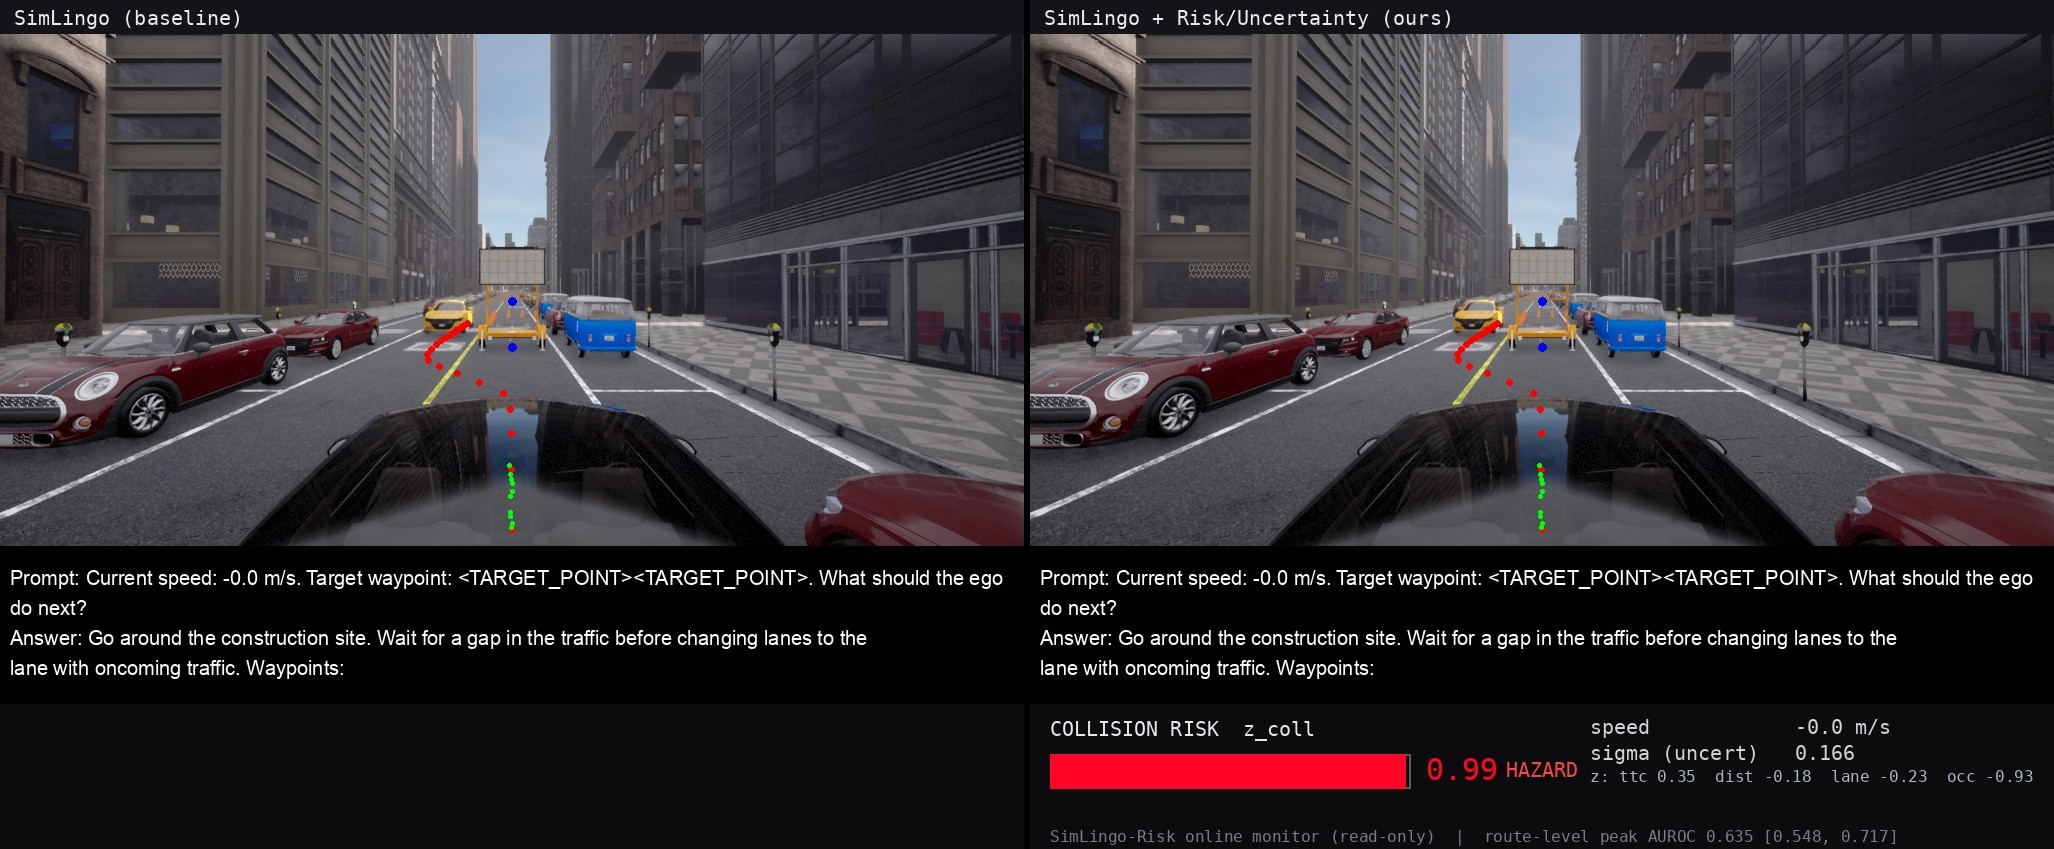
\includegraphics[width=\linewidth]{figures/construction.jpg}\\[-1pt]
{\footnotesize (a) Construction site ahead: $\zcoll=0.99$, $\sighat=0.166$}
\end{minipage}\hfill
\begin{minipage}{0.495\textwidth}\centering
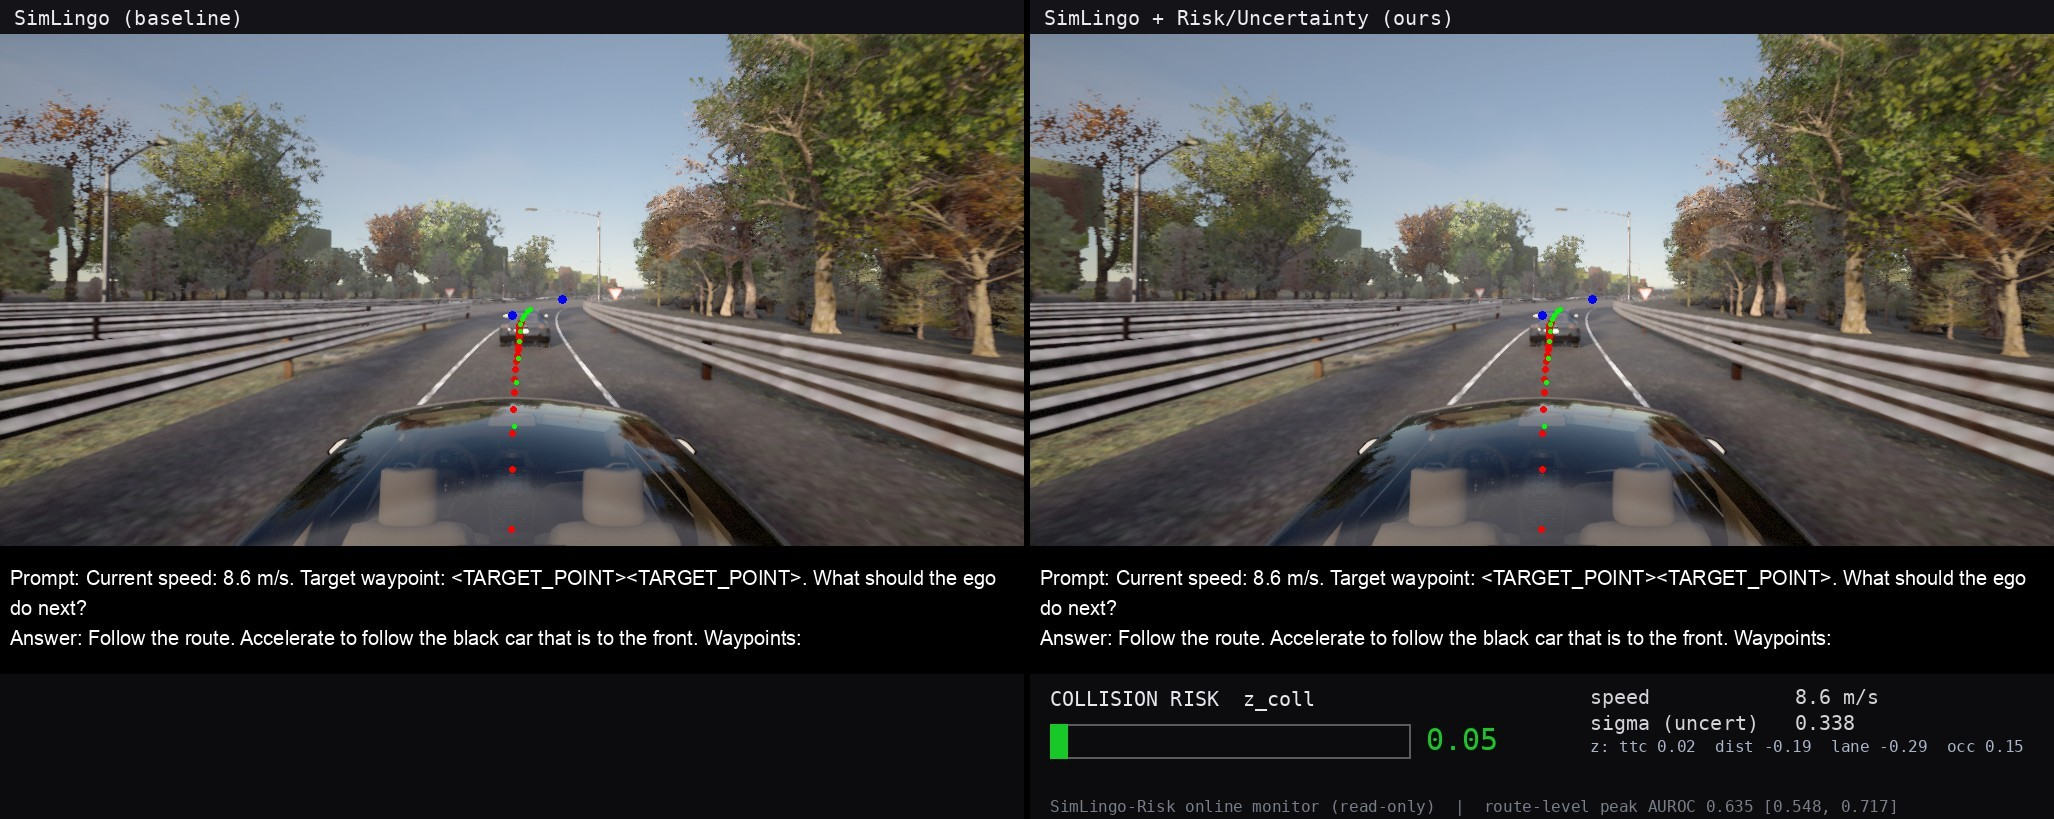
\includegraphics[width=\linewidth]{figures/following.jpg}\\[-1pt]
{\footnotesize (b) Following a lead car at speed: $\zcoll=0.05$, $\sighat=0.338$}
\end{minipage}
\caption{Risk and uncertainty are different axes. Each panel shows SimLingo as
published (left) and the same run with the monitor (right). (a) Clear danger and a
confident model. (b) Low risk and a less certain model.}
\label{fig:axes}
\end{figure*}

\begin{figure*}[t]
\centering
\begin{minipage}{0.495\textwidth}\centering
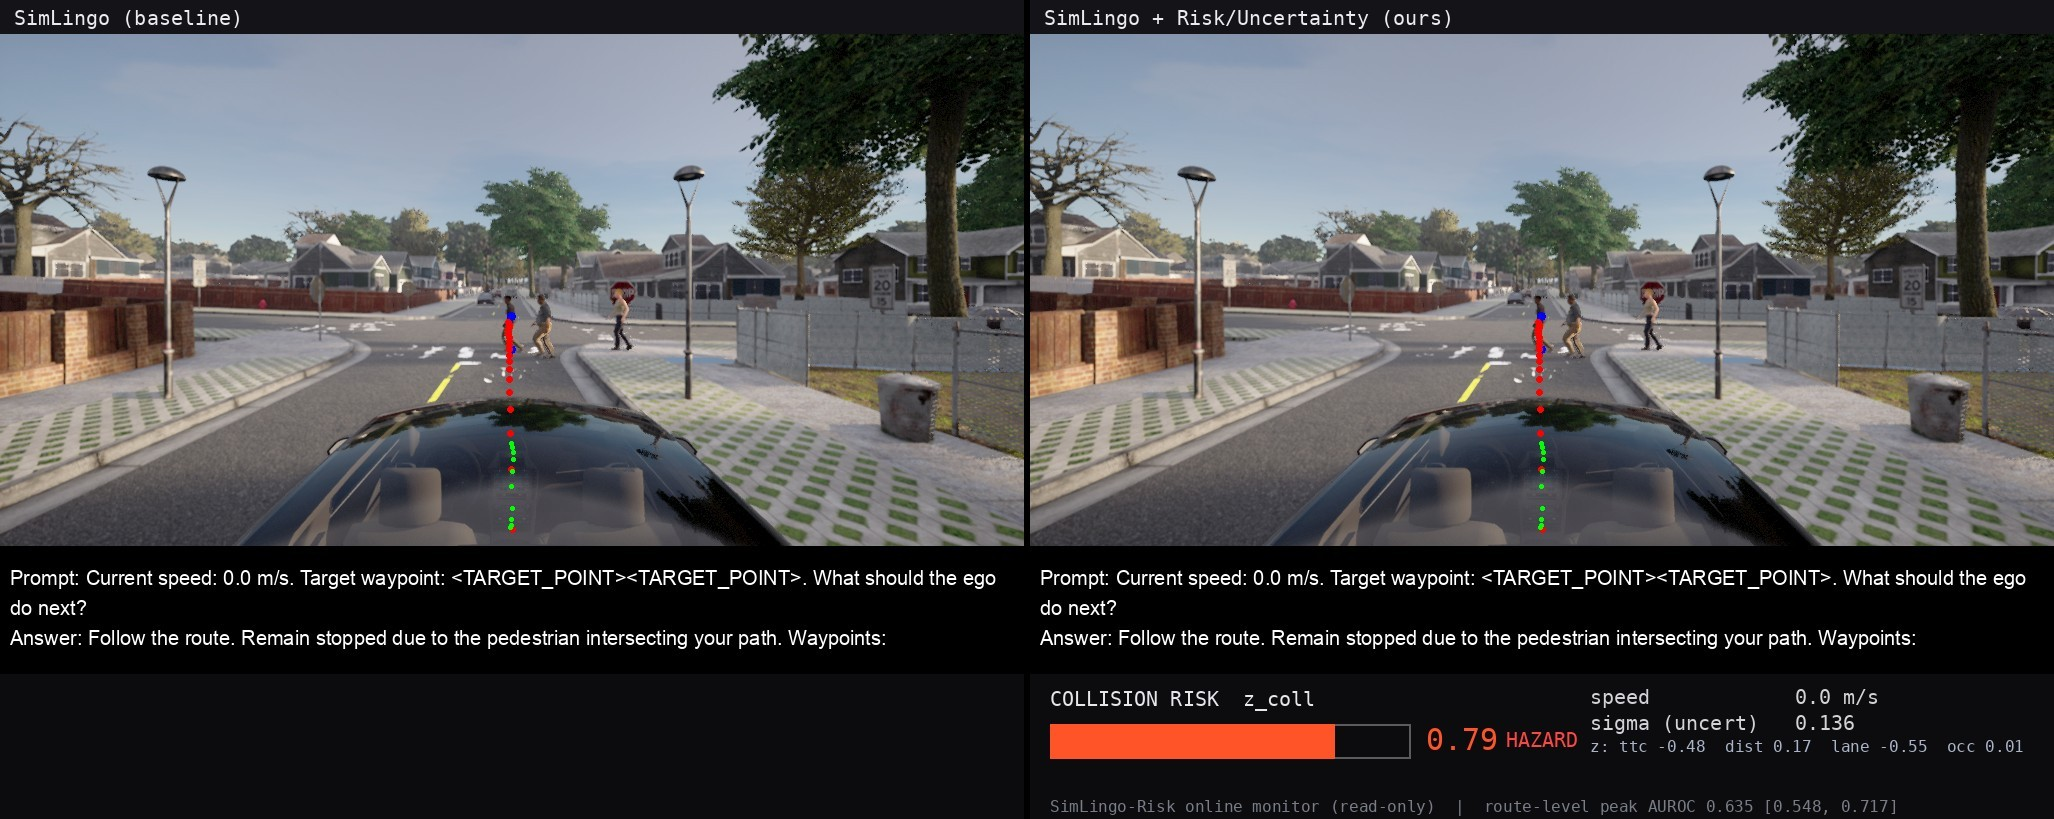
\includegraphics[width=\linewidth]{figures/pedestrians_day.jpg}\\[-1pt]
{\footnotesize (a) Pedestrians crossing, day: $\zcoll=0.79$, $\sighat=0.136$}
\end{minipage}\hfill
\begin{minipage}{0.495\textwidth}\centering
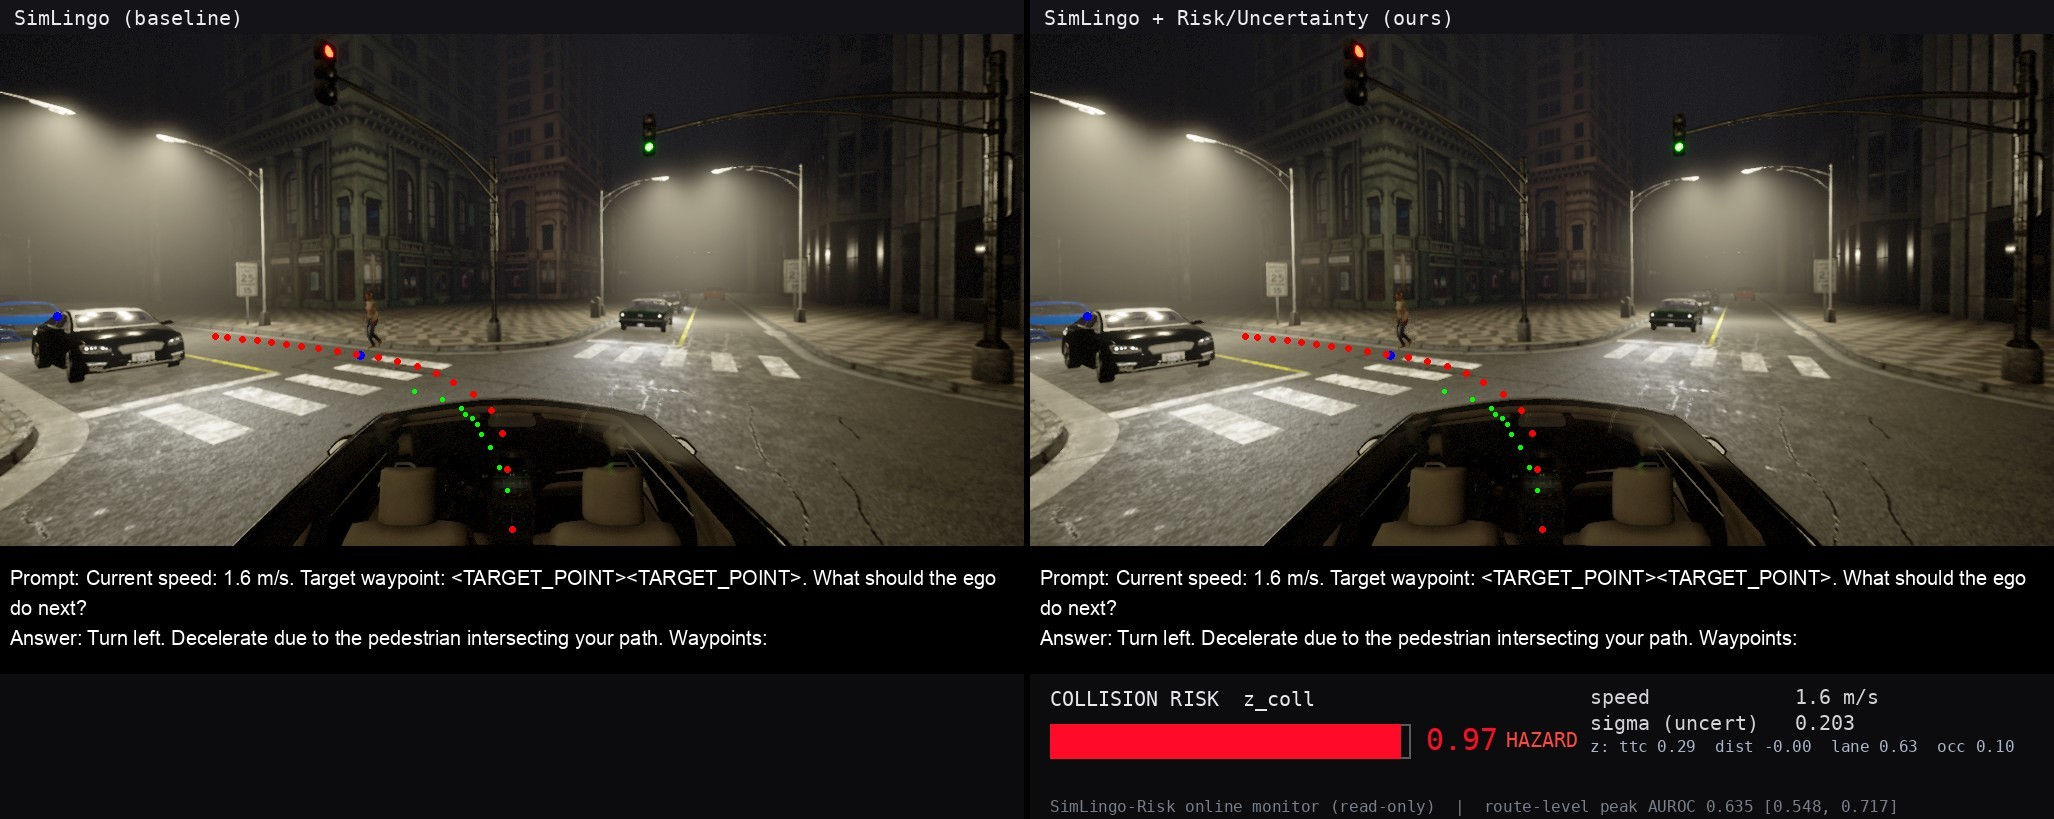
\includegraphics[width=\linewidth]{figures/pedestrian_fog.jpg}\\[-1pt]
{\footnotesize (b) Pedestrian crossing at night in fog: $\zcoll=0.97$,
$\sighat=0.203$}
\end{minipage}\\[6pt]
\begin{minipage}{0.495\textwidth}\centering
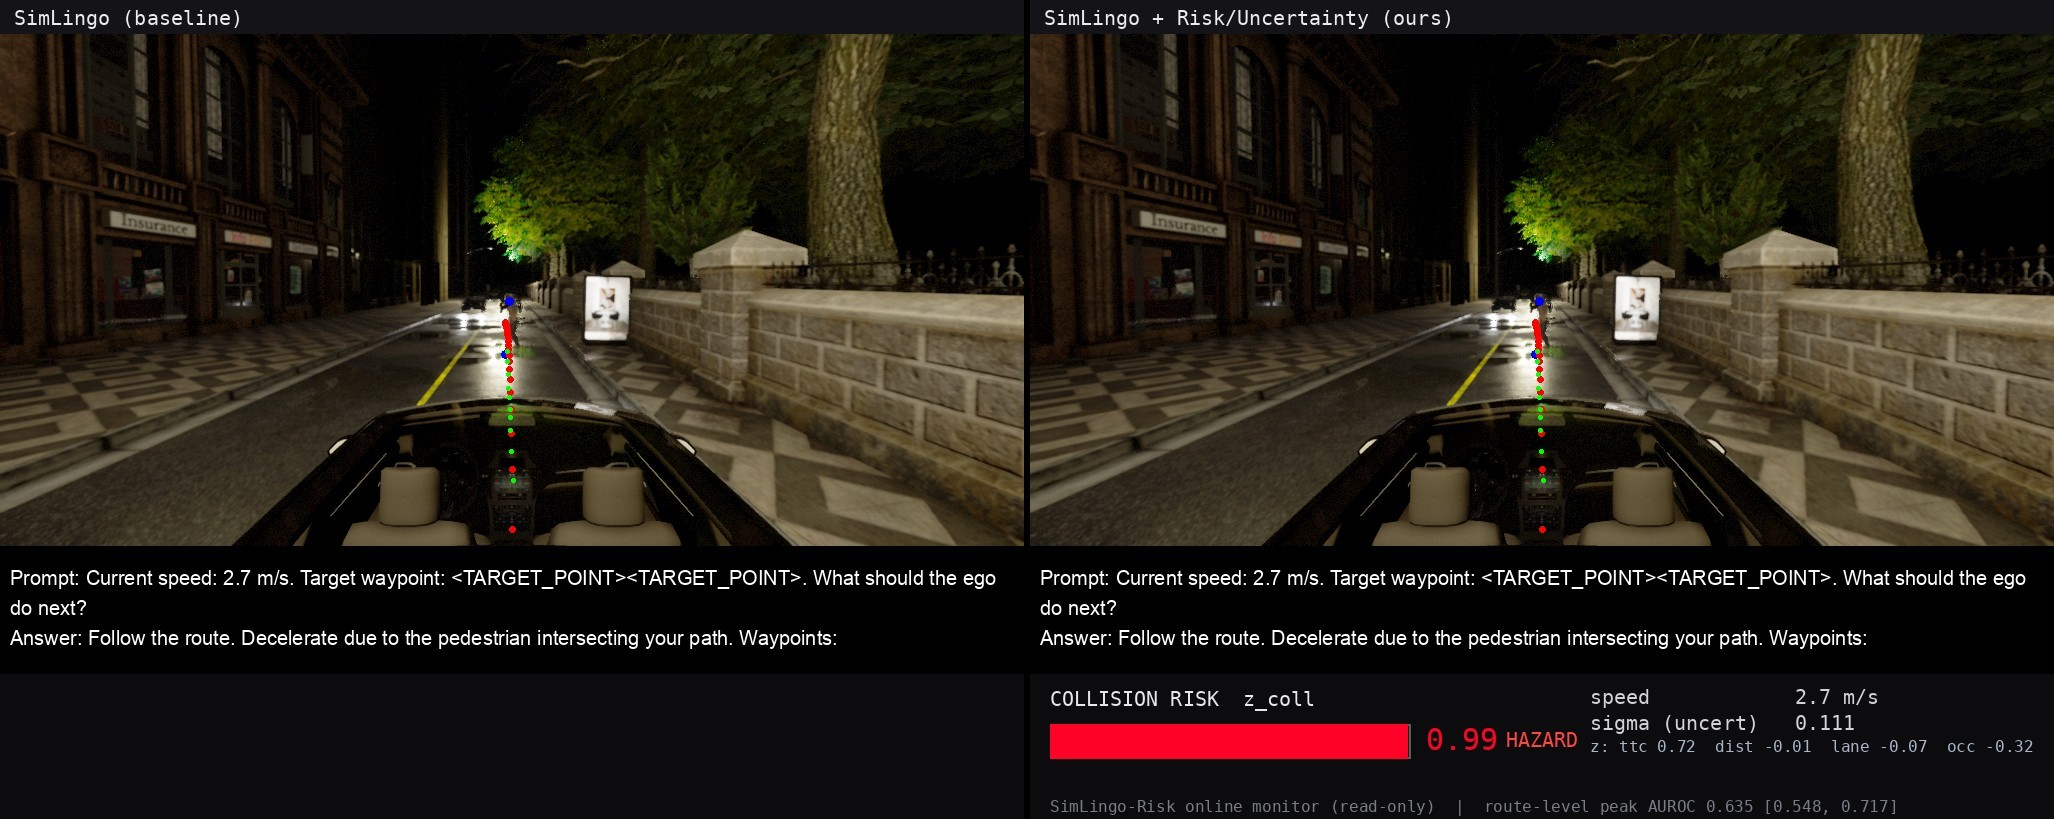
\includegraphics[width=\linewidth]{figures/pedestrian_night.jpg}\\[-1pt]
{\footnotesize (c) Pedestrian in the path at night: $\zcoll=0.99$,
$\sighat=0.111$}
\end{minipage}\hfill
\begin{minipage}{0.495\textwidth}\centering
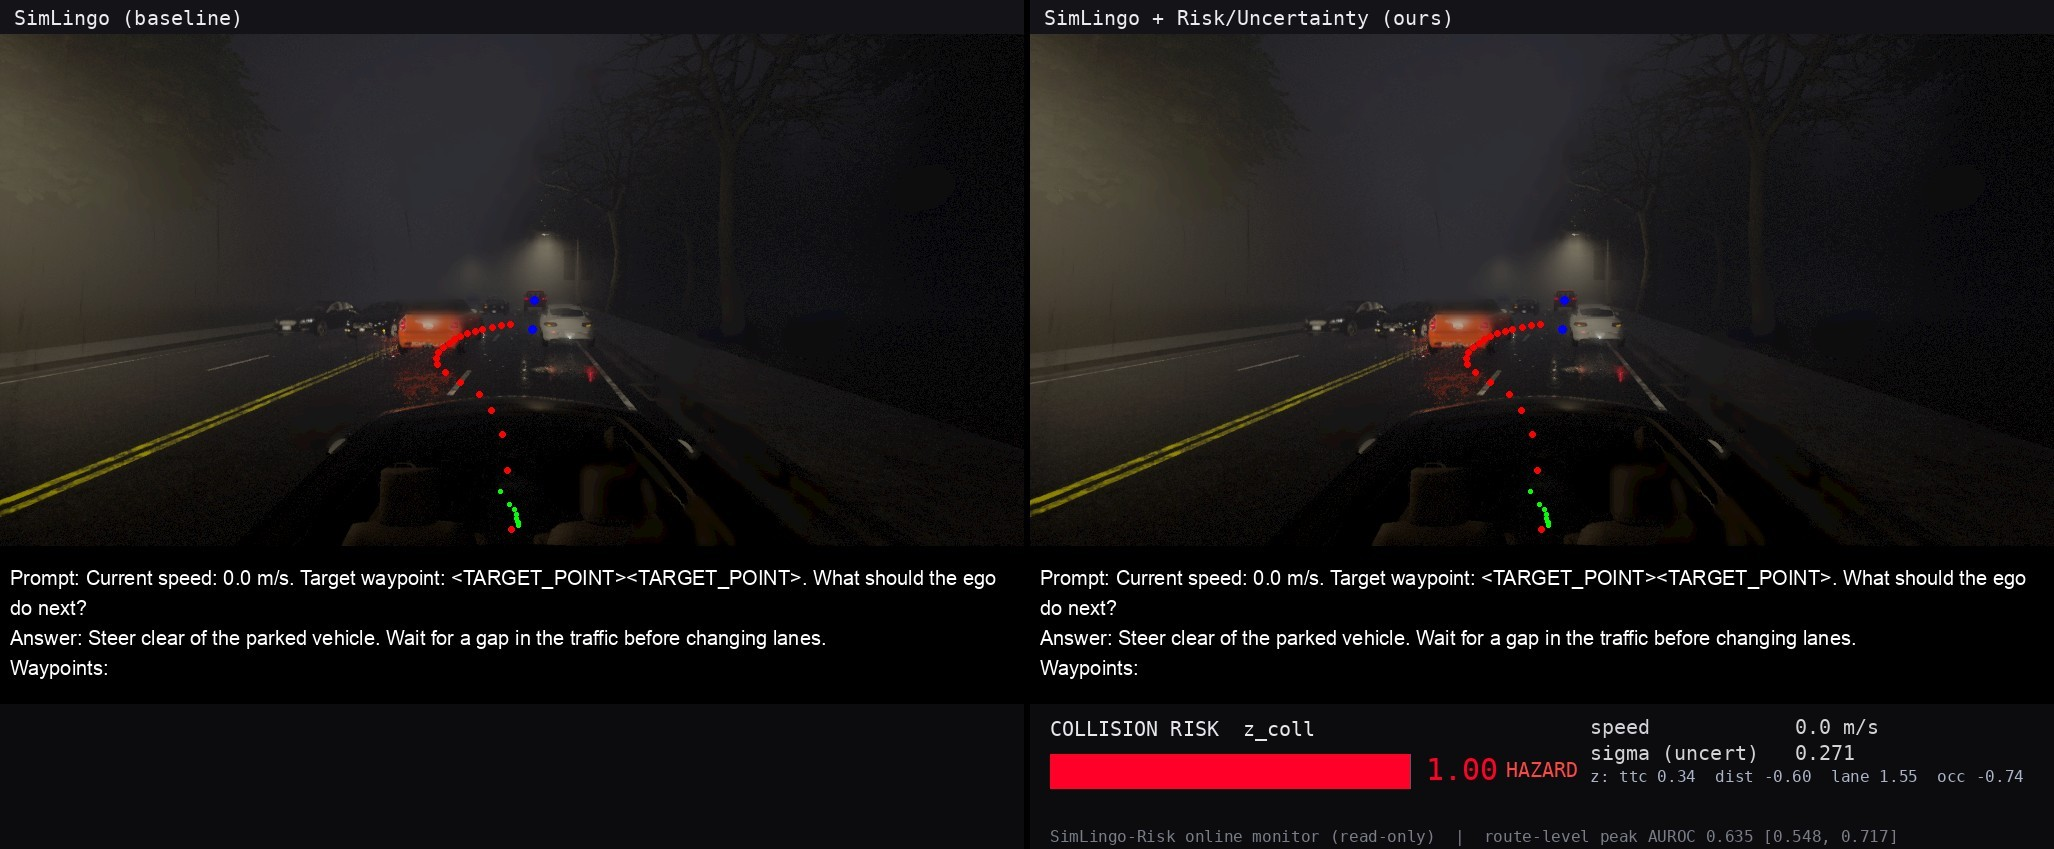
\includegraphics[width=\linewidth]{figures/parked_fog.jpg}\\[-1pt]
{\footnotesize (d) Parked vehicle in night fog: $\zcoll=1.00$, $\sighat=0.271$}
\end{minipage}
\caption{The monitor live in closed loop: SimLingo as published (left of each pair)
and the same run with the monitor (right). In each case SimLingo's own answer
already names the hazard (``Remain stopped due to the pedestrian'', ``Decelerate
due to the pedestrian'', ``Steer clear of the parked vehicle''); the monitor adds a
hazard score and an uncertainty.}
\label{fig:live}
\end{figure*}

\end{document}
